\begin{wrapfigure}{r}{0.6\textwidth}
	\vspace{-1.3cm}
	\centering
	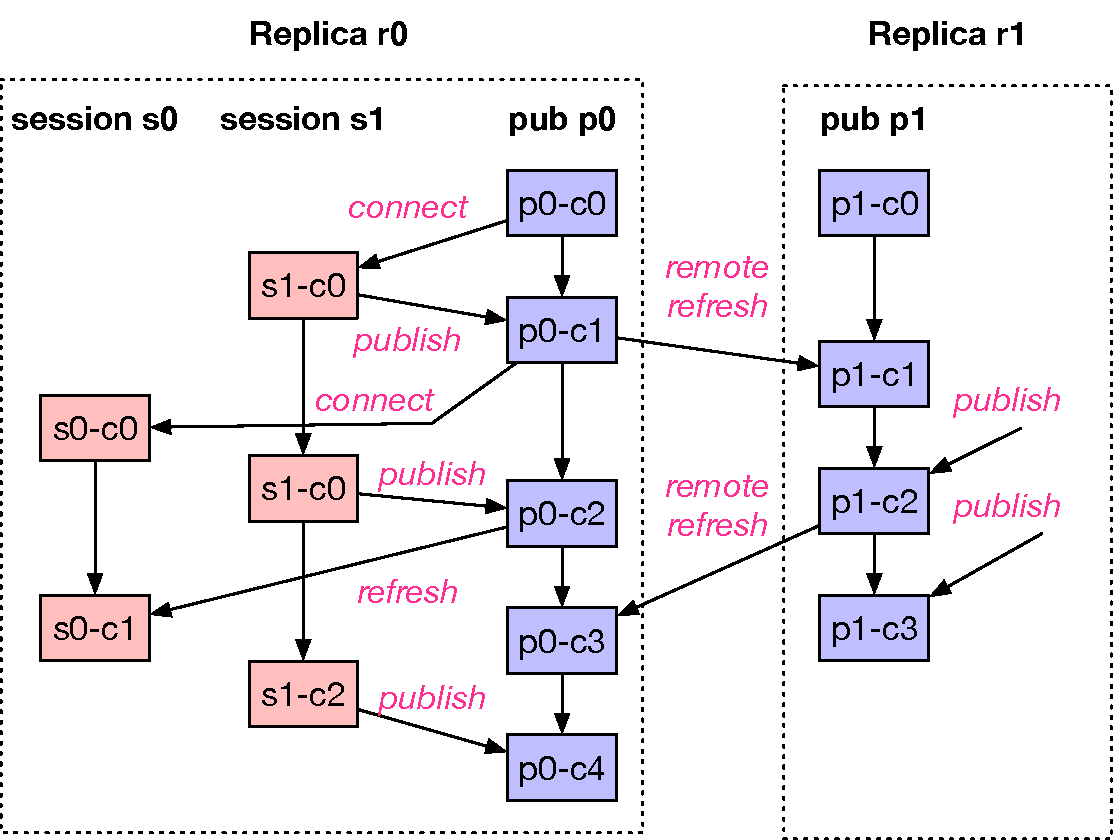
\includegraphics[scale=0.35]{figures/session_merge}
	\caption{\name system and programming model.}
	\vspace{-0.5cm}
	\label{fig:session_merge}
\end{wrapfigure}
In this section, we shall describe the system and programming model of \name
from the developers point-of-view. The \name store consists of several
replicas, which are fully or partially replicated~\cite{Crain15}. The replicas
asynchronously distribute updates amongst themselves until they converge. The
key property that enables \name to support mergeable types and isolated
transactions is that \name tracks the history of the store in the same way that
Git tracks the history of a repository.

Figure~\ref{fig:session_merge} presents the schematic diagram of the system and
programming model. Each replica has a distinguished public branch |pub|, which
records the history of the changing state at that replica. Each node in this
connected history graph represents a \emph{commit}. Whenever a new client
connection is established, a new branch is forked off the latest commit in the
public branch. Any reads or writes in this session is only committed to this
branch unless explicitly published. This ensures the isolation property of each
session. The figure shows the creation of two session in the replica |r0|.

The simplified \name API is given below:

\begin{lstlisting}
type config  (* Store configuration *)
type session
type key = string list
type value   (* Type of mergeable values in the store *)

val connect : config -> session Lwt.t
val close   : session -> unit Lwt.t
val read    : session -> key -> value option Lwt.t
val write   : session -> key -> value -> unit Lwt.t
val publish : session -> unit Lwt.t
val refresh : session -> unit Lwt.t
\end{lstlisting}

When a client connects to a \name store, a new session is created, which is
rooted to one of the replicas in the store. Every write creates a commit in the
session performing the write. As previously explained, \name permits the
sessions to atomically |publish| their updates and |refresh| to obtain latest
updates. The |publish| operation squashes all the local commits since the
previous |refresh| or |publish| to a single commit, and then \emph{pushes} the
changes to the public branch on the replica to which the session is rooted. The
|refresh| operation \emph{pulls} updates from the public branch into the
current sessions branch. Both |publish| and |refresh| may invoke the merge
function on the value type if there are conflicts. The objects that written to
each replica are asynchronously replicated to other replicas. \name offers
causal consistency for operations on each key.

Periodically, the changes from other public branches are \emph{pulled} into a
replica's public branch (remote refresh). This operation happens
\emph{implicitly} and asynchronously, and does not block the client on that
replica. When a session is closed, the outstanding writes are implicitly
published. Similarly, when a session is connected, there is an implicit refresh
operation.

Observe that both the local and the remote refresh operations are non-blocking
-- it is always safe for |refresh| to return with updates only from a subset of
public branches. The only push operation is due to |publish|. When pushing to a
branch, it is necessary to atomically update the target branch to avoid
concurrency errors. The key observation is that only the session that belongs
to a replica can push to the public branch on that replica. This can be
achieved with replica-local concurrency control and does not require
coordination among the replicas. Hence, \name transactions do not need
inter-replica coordination, and hence, are available.

When a particular replica goes down, the sessions that are rooted to that
replica may not have enough history to be able to |refresh| and |publish| to
other replicas. In particular, since |refresh| and |publish| will need to
discover the LCA in the case of conflicting updates. Since the objects are
asynchronously replicated across the replicas, the recent writes to the replica
that went down may not have been replicated to other replicas. Hence, \name
requires sticky availability~\cite{Bailis13} -- the sessions need to reach the
logical replica to which it originally connected. In practice, with partial
replication, a logical replica may be represented by a set of physical servers.
As long as one of these physical servers is reachable, the system remains
available for that session.

Compared to traditional transactions usually executed at a particular isolation
level, |refresh| and |publish| permits more fine-grained, explicit control of
visibility. In \name, transactions are delimited by |publish| operations, begin
and end of sessions. For example, the set of writes performed between
consecutive |publish| operations are made visible atomically outside the
session. The transaction may abort if the three-way merge function throws an
exception. However, in practice, the useful MRDTs are designed in such a way
that a merge is always possible, and the failure of the merge function
represents a bug. This idea of merge always being possible ensures \emph{strong
eventual consistency}, espoused by convergent replicated data
types~\cite{Shapiro11}. \name adds transactional support over strong eventual
consistency.

The |publish| and |refresh| can be used to achieve well-known isolation levels.
For example, snapshot isolation~\cite{Berenson95} is achieved by |refresh|ing
at that beginning of the transaction and |publish|ing at the end of the
transaction with no intervening |refresh|es. Unlike snapshot isolation, the
conflicting updates will be resolved with the three-way merge function. If two
consecutive |publish| operations are interspersed with |refresh|es, then one
gets the monotonic atomic view~\cite{Bailis13} isolation level.
